\section{Interaktions-Seite [M]}
\setauthor{Fabian Maar}

\subsection{Bewegung}
Um sich im Ausstellungsraum bewegen zu können, ist es nötig, den Besuchern*innen eine entsprechende Fortbewegungsmöglichkeit zu bieten. Three.js implementiert diese Funktion mittels Controls. Im Endeffekt ändert sich die Position und Rotation der Kamera durch Benutzereingaben. Die wesentlichsten Controls in Three.js sind

\begin{itemize}
    \item DragControls - Der*die Nutzer*in kann sich mittels DragNDrop Interaktionen fortbewegen \cite{DragControls}
    \item FirstPersonControls - Der*die Nutzer*in bewegt sich wie in einem Videospiel mit den Tasten W, A, S und D fort. Dabei ist es möglich, das Blickfeld über die Maus zu steuern. \cite{FirstPersonControls}
    \item OrbitControls - Der*die Nutzer*in kann mittels linker Maustaste um ein bestimmtes Ziel kreisen. Durch die rechte Maustaste kann dieses Ziel geändert werden. \cite{OrbitControls}
    \item //TODO
\end{itemize}


\subsection{Border-Collision}
Um den Benutzern*innen ein möglichst realistisches Gefühl für die Ausstellung zu geben, ist es wichtig, den Ausstellungsraum authentisch zu gestalten. Daher ist der Raum durch Wände abgegrenzt, wodurch es nicht mehr möglich ist, sich über den Raum hinaus zu bewegen. Um eine Kollision mit der Wand zu berechnen, gibt es durch die Three.js Bibliothek einige Möglichkeiten.

\subsection{Bounding Box}
Der erste Ansatz der Umsetzung war das Erstellen einer Bounding Box. Dabei kann zwischen zwei verschiedenen Arten unterschieden werden. 

\begin{itemize}
    \item Axis Aligned Bounding Box (AABB)
    \newline
    Zum einen werden Axis Aligned Bounding Box verwendet, um eine Box rund um das 3D-Objekt zu erstellen, die sich nicht an die Rotation des Objekts anpasst.
    \item Oriented Bounding Box (OBB)
    \newline
    Die Oriented Bounding Box funktioniert im Endeffekt gleich, unterscheidet sich aber darin, dass sie sich an die Achsen des Objekts anpasst
    
    Da sich die Bounding Boxen jedoch über den ganzen 3D-Raum erstrecken, wird eine Kollision direkt berechnet, nachdem der*die Benutzer*in den Raum betritt. Da sich die Bounding Boxen nicht an jede einzelne Wand anpassen konnten, musste ein anderer Lösungsweg gefunden werden.
\end{itemize}
\begin{figure}
    \centering
    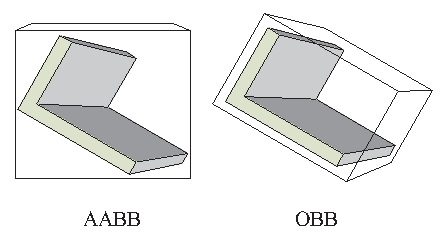
\includegraphics[scale=0.65]{pics/aabb_obb.png}
    \caption{Der Unterschied zwischen AABB und OBB \cite{AABBandOBBPicture}}
    \label{fig:impl:aabb_obb}
\end{figure}


\subsubsection{Zweiter Ansatz}
Um eine Veränderung der Position des*der Benutzers*in festzustellen, muss die Veränderung der Kameraposition evaluiert werden.Bei der Initialisierung der Kamera wird eine Kopie erstellt. In der Animate-Funktion wird eine Veränderung der Kamera überprüft, indem die Positionen der Kamera mit der Kopie verglichen werden. Die Kamera nimmt dabei immer eine neue Position ein, wenn sich der*die Benutzer*in im Raum bewegt, während die Kopie dabei die alte Position der Kamera einnimmt. Jedes Mal wenn eine Veränderung geschieht, wird überprüft, ob die Kamera mit der Wand kollidiert. Dies geschieht, indem ein Raycast mit den Positionen der Kamera und der Kopie initialisiert wird. 
     
\subsubsection{Far und Near}
Die Attribute Far und Near werden dafür verwendet, um die Objekte, die im Ray liegen, einzugrenzen. Dies wird durch die Methode des Clippings realisiert //TODO Referenz. Dabei können die Werte nicht negativ sein und der Far-Wert muss größer als der Near-Wert sein. Um die Kollision erst direkt am Ursprungsort, im Falle der Kamera, des Rays zu berechnen, wird der Far-Wert auf 100 gesetzt.
   	
Nachdem der Raycast //TODO Referenz korrekt initialisiert und angewandt wurde, muss bei einer Berührung mit der Wand nur noch richtig damit umgegangen werden. Dabei wird die Bewegung des Benutzers gestoppt. Um diese auch wieder zu starten, muss sich der*die Benutzer*in weg von der Wand begeben. Überprüft wird dies nach jeder Benutzer*inneneingabe mit einem Event-Listener. Falls nach dieser keine Berührung mehr mit einer Wand besteht, wird die Bewegung fortgesetzt und der*die Besucher*in kann sich wieder frei im Raum bewegen.

\newpage

